%! TeX program = xelatex
\documentclass{beamer}

%% PACKAGES %%

% Macro making packages
\usepackage{xparse}
\usepackage{xpatch}
\usepackage{tokcycle}

% Standalone compilation
\usepackage[obeyclassoptions,mode=tex]{standalone}

% Math typesetting 
\usepackage{amsmath}
\usepackage{amsthm}
\usepackage{thmtools}
\usepackage{upgreek}
\usepackage{amssymb}
\usepackage{stmaryrd}

% References and knowledge management
\usepackage{hyperref}
\usepackage[capitalise,noabbrev,nameinlink]{cleveref}
\usepackage[electronic,hyperref,xcolor,cleveref]{knowledge}
\knowledgeconfigure{notion}

% BIBTEX / BIBLATEX
\usepackage[
	%style=numeric-comp,
    %citestyle=authortitle-icomp,
	citestyle=numeric-comp,
	%bibstyle=authoryear,
	bibstyle=numeric,
	%sorting=none,
    sorting=nyt,
	%sortcites=true,
	%autocite=footnote,
    maxnames=99,
    %backend=biber, % Compile the bibliography with biber
    backend=bibtex,
    %refsegment=chapter, % split references ?
	hyperref=true,
	backref=true,
	citecounter=true,
	pagetracker=true,
	citetracker=true,
	ibidtracker=context,
	autopunct=true,
	autocite=plain,
    doi=true,
]{biblatex}

% Table typesetting
\usepackage{booktabs}
\usepackage{varwidth}

% Proofs typesetting
\usepackage{bussproofs}

% Drawing
\usepackage{tikz}
\usetikzlibrary{backgrounds}
\usetikzlibrary{shapes.geometric}
\usetikzlibrary{positioning}
\usetikzlibrary{automata}
\usetikzlibrary{tikzmark}
\usetikzlibrary{patterns}
\usetikzlibrary{arrows}
\usepackage{tikz-cd}
\tikzset{every state/.style={minimum size=1pt}}

% ENS PARIS SACLAY COLORSCHEME
\definecolor{Prune}{RGB}{99,0,60}
\definecolor{A1}{HTML}{000000}
\definecolor{B1}{RGB}{49,62,72}
\definecolor{C1}{RGB}{124,135,143}
\definecolor{D1}{RGB}{213,218,223}
\definecolor{A2}{RGB}{198,11,70}
\definecolor{B2}{RGB}{237,20,91}
\definecolor{C2}{RGB}{238,52,35}
\definecolor{D2}{RGB}{243,115,32}
\definecolor{A3}{RGB}{124,42,144}
\definecolor{B3}{RGB}{125,106,175}
\definecolor{C3}{RGB}{198,103,29}
\definecolor{D3}{RGB}{254,188,24}
\definecolor{A4}{RGB}{0,78,125}
\definecolor{B4}{RGB}{14,135,201}
\definecolor{C4}{RGB}{0,148,181}
\definecolor{D4}{RGB}{70,195,210}
\definecolor{A5}{RGB}{0,128,122}
\definecolor{B5}{RGB}{64,183,105}
\definecolor{C5}{RGB}{140,198,62}
\definecolor{D5}{RGB}{213,223,61}


\foreach \name in {A,B,C,D} {
    \foreach \hue in {1,2,3,4,5} {
        \foreach \shade/\intensity in {hint/20,bg/50} {
            \xglobal\colorlet{\name\hue\shade}{\name\hue!\intensity!white}
        }
    }
}

\newcommand{\tableofcolors}{
    \begin{tikzpicture}
        \foreach \letter/\x in {A/0,B/1,C/2,D/3} {
            \foreach \y/\variant in {0/1,1/2,2/3,3/4,4/5} {
                \node[color=\letter\variant] (\letter\variant) at (\x,\y) {\letter\variant};
                \node[color=\letter\variant bg]
                    (BG\letter\variant) at ({\x - 0.2}, {\y - 0.2}) {\letter\variant};
                \node[color=\letter\variant hint] 
                    (HT\letter\variant) at ({\x - 0.4}, {\y - 0.4}) {\letter\variant};
            }
        }
        \begin{scope}[xshift=2cm]
            \foreach \name/\x/\y in {
                Prune/3/4
            } {
                \node[color=\name] (\name) at (\x,\y) {\name};
            }

        \end{scope}
    \end{tikzpicture}
}


\usetheme[sectionpage=none,subsectionpage=progressbar]{metropolis}
\usepackage{appendixnumberbeamer}
\usepackage[toc,page]{appendix}

\usepackage[no-math]{fontspec}
\setmainfont{Roboto}
\setsansfont{Andika}
\setmonofont{Ubuntu Mono}


% knowledge management
\knowledgestyle{intro notion}{color={A5}, emphasize}
\knowledgestyle{notion}{color={A4}}
\knowledgeconfigure{anchor point color={A2},
                    anchor point shape=corner}
\knowledgestyle{intro unknown}{color={D3}, emphasize}
\knowledgestyle{intro unknown cont}{color={C3}, emphasize}
\knowledgestyle{kl unknown}{color={D2}}
\knowledgestyle{kl unknown cont}{color={C2}}

\hypersetup{
    colorlinks=true,
    anchorcolor=A2,
    citecolor=A4,
    linkcolor=A4,
    urlcolor=A3,
    filecolor=A3,
    runcolor=D2,
    menucolor=D2,
}

\NewDocumentCommand{\klscope}{ o m }{
    \withkl{\kl[#1]}{#2}
}

% Common theorem styles
\theoremstyle{plain}
\newtheorem{conjecture}[theorem]{Conjecture}


% Upgreek letters
\makeatletter
\newcommand\mathgr[1]{\tokcycle
  {\addcytoks{##1}}
  {\processtoks{##1}}
  {\ifcsname up\expandafter\@gobble\string##1\endcsname
   \addcytoks[1]{\csname up\expandafter\@gobble\string##1\endcsname}%
    \else\addcytoks{##1}\fi}
  {\addcytoks{##1}}{#1}%
  \expandafter\mathrm\expandafter{\the\cytoks}%
}
\makeatother

% Comment on a definition/text
\NewDocumentCommand{\comment}{m}{%
    \footnote{#1}%
}

% Citation configuration
\AtEveryBibitem{
    % Removes issn, isbn, and
    % unwanted items from the bibliography
	\clearfield{issn}
	\clearfield{isbn}
	\clearfield{archivePrefix}
	\clearfield{arxivId}
	\clearfield{pmid}
	\clearfield{eprint}
}

% Cite a knowledge
\NewDocumentCommand{\citek}{ o m }{
    \IfNoValueTF{#1}{
        \cite{m}
    }{
        \cite[{\kl(#1)[#2]}]{#1}
    }
}

%
% Here are the definitions
% of mathematical macros.
%
%

\newcommand{\defined}{:=}


\NewDocumentCommand{\Paths}{}{\mathsf{Paths}}
\NewDocumentCommand{\Cycles}{}{\mathsf{Cycles}}

\NewDocumentCommand{\FO}{}{\mathsf{FO}}
\NewDocumentCommand{\EFO}{}{\mathsf{EFO}}
\NewDocumentCommand{\MSO}{}{\mathsf{MSO}}

\newcommand{\Neighb}[3]{\mathcal{N}_{#1}(#2, #3)}
\newcommand{\Loc}[3]{\mathsf{Loc}(#1,#2, #3)}

\newcommand{\Nat}{\mathbb{N}}

\newcommand{\setof}[2]{\{ #1 \mid #2 \}}
\newcommand{\set}[1]{\{ #1 \}}

\NewDocumentCommand{\isubleq}{}{\mathrel{\subseteq_i}}

\NewDocumentCommand{\model}{m}{\mathfrak{#1}}

\NewDocumentCommand{\aPath}{m}{\mathsf{P}_{#1}}
\NewDocumentCommand{\aCycle}{m}{\mathsf{C}_{#1}}
\NewDocumentCommand{\aClique}{m}{\mathsf{K}_{#1}}

\NewDocumentCommand{\upset}{ m }{\mathop{\uparrow}#1}

\NewDocumentCommand{\modset}{ O{} m }{\llbracket #2 \rrbracket_{#1}}


\NewDocumentCommand{\restr}{ m m }{ {#1}_{|#2}}

\input{globals/knowledges.kl}

\title{Locality and the Łoś–Tarski Theorem \\ (in Finite Model Theory)}
\subtitle{A combinatoric tale}

\author{Aliaume LOPEZ}
\date{8 February 2024}

\institute{
    LIRMM AlgCo Seminar
    \begin{center}
        
\includegraphics[height=3em]{images/universite_paris_saclay.pdf}
        \hspace{1em}
        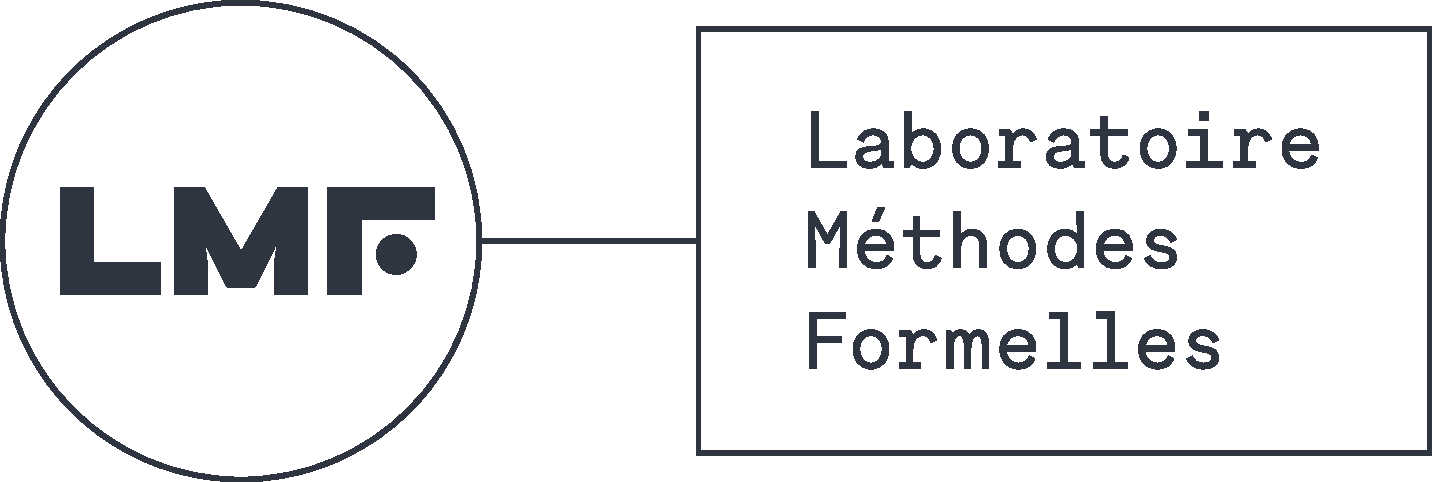
\includegraphics[height=3em]{images/lmf-logo.pdf}
        \hspace{1em}
        
\includegraphics[height=3em]{images/irif.pdf}
        \hspace{1em}
        
\includegraphics[height=3em]{images/universite_paris_cite.pdf}
    \end{center}
}

\bibliography{globals/papers}


\newcommand{\tightlist}{}

\begin{document}

\begin{frame}
    \maketitle
\end{frame}

\begin{frame}{Guessing Game}
    \begin{center}
        \foreach[count=\xi] \i in {1,...,5} {
            \only<\xi>{
                \includegraphics[width=15cm]{figures/quizz_Page \i.png}
            }
        }
    \end{center}
\end{frame}

\begin{frame}{Guessing Game for monotone sentences}
    \begin{lemma}
        \vspace{0.1em}
        For every non-trivial sentence $\varphi$,
        the following are equivalent:
        \begin{enumerate}
            \item $\varphi \equiv \exists^{\geq n} x. \top$ over $\Paths$;
            \item $\varphi$ is \textbf{monotone} over $\Paths$;
            \item The set of models of $\varphi$ (in $\Paths$)
                is described using a single element.
        \end{enumerate}
    \end{lemma}
    \pause
    \begin{alertblock}{New item found!}
        \vspace{0.1em}
        \centering
        This is the Łoś-Tarski Theorem (for $\Paths$).
    \end{alertblock}
\end{frame}

\section{Preservation Theorems}
\subsection{What, why, and where?}

\begin{frame}{Monotonicity}
    \begin{definition}[Induced Substructure]
        \vspace{0.1em}
        Existence of a \textbf{strong} \textbf{injective} \textbf{homomorphism}
        between structures $\model{A}$ and $\model{B}$:
        \begin{equation*}
            \model{A} \isubleq \model{B} 
        \end{equation*}
    \end{definition}
    \begin{center}
        \foreach[count=\xi] \i in {6,7,8} {
            \only<\xi>{
                \includegraphics[width=11cm]{figures/quizz_Page \i.png}
            }
        }
    \end{center}
\end{frame}

\begin{frame}{Induced substructures}
    \begin{block}{Comparing paths, cycles, cliques ...}
        \begin{itemize}
            \item For finite paths, $\aPath{n} \isubleq \aPath{m} \iff n \leq m$
            \item For finite cycles, $\aCycle{n} \isubleq \aCycle{m} \iff n = m$
            \item For finite cliques, $\aClique{n} \isubleq \aClique{m} \iff n \leq m$.
        \end{itemize}
    \end{block}
\end{frame}

\begin{frame}{Formulas}
    \begin{block}{The logic $\FO$ and its existential fragment $\EFO$}
        \begin{equation*}
        \varphi := \underbrace{\varphi \wedge \varphi
                \mid \varphi \vee \varphi
                \mid \neg R(\vec{x})
                \mid R(\vec{x})
                \mid \exists x. \varphi
                }_{\onslide<2->{\EFO}}
                \onslide<2->{\color{B2}
                 \mid \forall x. \varphi}
        \end{equation*}
    \end{block}
    \pause\pause
    \begin{equation*}
        \underbrace{
            \exists x. \neg B(x)
        }_{\onslide<4>{\in} \EFO}
        \quad \quad
        \underbrace{\forall x. B(x)
        }_{\onslide<4>{\not\in} \EFO}
    \end{equation*}
\end{frame}

\begin{frame}{Drawing conventions}
    \begin{center}
        \foreach[count=\xi] \i \in {9,10,11} {
            \only<\xi>{
                \includegraphics[width=15cm]{figures/quizz_Page \i.png}
            }
        }
    \end{center}
\end{frame}

\begin{frame}{The Łoś-Tarski Theorem}
    \begin{theorem}[{\cite{TARSKI57,LOS55}}]
        \vspace{0.1em}
        For every first order
        sentence \(\varphi\), the following are equivalent:
        \begin{enumerate}
        \item
            \(\varphi\) is \emph{preserved under extensions}
            \hfill
            (\textbf{monotone} for $\isubleq$)
        \item
          \(\varphi\) is equivalent to an existential sentence
          \hfill
          ($\varphi \equiv \psi$ for some $\psi \in \EFO$)
        \item
          \(\varphi\) is the \(\subseteq_i\)-upwards closure of finitely many
          \emph{finite} models
          \hfill
          ($\modset{\varphi} = \upset{\model{A}_1, \dots, \model{A}_n}$)
        \end{enumerate}
    \end{theorem}
    \pause
    Note that the only difficult implication of the theorem is (1) implies
    (2/3).
    \pause
    \begin{alertblock}{!! Over the class of all structures !!}
    \end{alertblock}
\end{frame}

\subsection{Theoretical implications?}\label{theoretical-implications}

\begin{frame}{Theoretical implications?}

    Using the \textbf{Homomorphism Preservation Theorem}
    (variation of the Łoś--Tarski Theorem).

    \textbf{\autocite[Proposition 1]{LIBK11}.} Naïve evaluation of a query
    \(q\) computes its \emph{certain answers} if and only if \(q\) is a
    union of conjunctive query.

    \textbf{\autocite[Theorem 17]{DENJ08}.} The \emph{core chase} terminates
    on an initial database \(I\) and constraints \(\Sigma\) if and only if
    \(\mathop{\uparrow}(\Sigma \cap I)\) is first-order definable.

\end{frame}

\subsection{In the finite?}\label{in-the-finite}

\begin{frame}{Łoś-Tarski in the finite?}

\begin{longtable}[]{@{}
  >{\raggedright\arraybackslash}p{(\columnwidth - 2\tabcolsep) * \real{0.7614}}
  >{\raggedright\arraybackslash}p{(\columnwidth - 2\tabcolsep) * \real{0.2386}}@{}}
\toprule\noalign{}
\begin{minipage}[b]{\linewidth}\raggedright
Class of Structures
\end{minipage} & \begin{minipage}[b]{\linewidth}\raggedright
Relativisation
\end{minipage} \\
\midrule\noalign{}
\endhead
All finite structures & NO \autocite{TAIT59} \\
\(\emptyset\) & YES \\
Bounded tree-depth & YES \autocite{wqo:DING92} \\
Cycles & NO \\
Paths & YES \\
Cliques & YES \\
Bounded degree, hereditary, and closed under disjoint unions & YES
\autocite{ADG08} \\
Planar Graphs & NO \autocite{ADG08} \\
\bottomrule\noalign{}
\end{longtable}
\end{frame}

\subsubsection{What are the tools?}\label{what-are-the-tools}

\begin{frame}{The proof scheme.}
\protect\hypertarget{the-proof-scheme.}{}
Given a sentence \(\varphi\) preserved under extensions over a class
\(\mathcal{C}\), do the following:

\begin{enumerate}
\tightlist
\item
  Rewrite \(\varphi\) as a Boolean combination of ``basic local
  sentences'' \autocite{GAIF82}
\item
  Assume by contradiction that \(\varphi\) has arbitrarily large
  \(\subseteq_i\)-minimal models
\item
  In large enough minimal models, neighbourhoods ``repeat'' a lot, and
  can be ``contracted''
\item
  Obtain a contradiction because \(\varphi\) cannot observe the
  contraction
\end{enumerate}
\end{frame}

\subsection{The best ``generic'' result prior to this work}

\begin{frame}{The best ``generic'' result prior to this work}
\textbf{Theorem \autocite{ADG08}.} Let \(\mathcal{C}\) be a hereditary
class of finite structures closed under disjoint unions. If
\(\mathcal{C}\) has \emph{bounded degree}, then the Łoś--Tarski Theorem
relativises to \(\mathcal{C}\).

\textbf{Remark.} Hereditary means that existential sentences are
precisely those with finitely many minimal models.
\end{frame}

\section{The results}\label{the-results}

\subsection{Localisations}\label{localisations}

\begin{frame}{Main theorem}
\textbf{Theorem.} For every \emph{hereditary} class \(\mathcal{C}\) of
finite structures that is closed under disjoint unions, the following
are equivalent

\begin{enumerate}
\tightlist
\item
  The Łoś--Tarski Theorem relativises to \(\mathcal{C}\).
\item
  The Łoś--Tarski Theorem relativises to all \textbf{localisations} of
  \(\mathcal{C}\).
\end{enumerate}

\textbf{Remarks.}

\begin{itemize}
\tightlist
\item
  Strictly generalises \autocite{ADG08}
\item
  Is now an equivalence
\item
  Yields new classes of structures
\end{itemize}
\end{frame}

\begin{frame}{What is a neighbourhood?}
\(\mathcal{N}_{A}(\vec{a}, r)\)
\end{frame}

\subsubsection{Example of
neighbourhoods}\label{example-of-neighbourhoods}

\subsubsection{What is a localisation?}\label{what-is-a-localisation}

\begin{frame}{What is a localisation?}
\(\mathsf{Loc}(\mathcal{C},k, r) := \{ \mathcal{N}_{A}(\vec{a}, r) \mid  \vec{a} \in A^k \}\)

\textbf{Remark.}
\(\mathcal{C} = \bigcup_{k,r} \mathsf{Loc}(\mathcal{C},k, r)\)
\end{frame}

\subsubsection{Example of localisations}\label{example-of-localisations}

\begin{frame}{Example of localisations}
\begin{itemize}
\tightlist
\item
  Bounded degree iff localisations are finite
\item
  Cycles -\textgreater{} localisation contains finitely many cycles!
\item
  Cliques -\textgreater{} localitasions are the whole class at every
  step
\end{itemize}
\end{frame}

\subsubsection{How do we use such a
theorem?}\label{how-do-we-use-such-a-theorem}

\begin{frame}{How do we use such a theorem?}
COPY FIGURE ABOUT NEW CLASSES
\end{frame}

\section{The proofs}\label{the-proofs}

\subsection{Positive Locality and
Neighbourhroods}\label{positive-locality-and-neighbourhroods}

\subsubsection{Local formulas}\label{local-formulas}

\begin{frame}{Local formulas}
A formula is local if its truth value only depends on the local
neighbourhood of the free variables.
\end{frame}

\subsubsection{Local sentences?}\label{local-sentences}

\begin{frame}{Local sentences?}
Does not make sense to consider local sentences (either true or false)
\end{frame}

\subsubsection{Basic local sentences}\label{basic-local-sentences}

\begin{frame}{Basic local sentences}
Gaifman defined basic local sentences as follows:
\end{frame}

\subsubsection{Existential local
sentences}\label{existential-local-sentences}

\begin{frame}{Existential local sentences}
Another way to define local sentences is to consider existential
quantification of local formulas.

\textbf{Remark.} \(0\)-local is existential, \(\infty\)-local is
arbitrary formulas.
\end{frame}

\subsubsection{Positive Locality}\label{positive-locality}

\begin{frame}{Positive Locality}
\textbf{Theorem \autocite{GAIF82}.} Every sentence \(\varphi\) is
equivalent to a Boolean combination of basic local sentences.

\textbf{Theorem.} For every sentence \(\varphi\), the following are
equivalent:

\begin{enumerate}
\tightlist
\item
  \(\varphi\) is equivalent to a \textbf{positive} Boolean combination
  of basic local sentences.
\item
  \(\varphi\) is equivalent to an existential local sentence.
\end{enumerate}
\end{frame}

\subsection{Combinatorics of
Neighbourhroods}\label{combinatorics-of-neighbourhroods}

\subsubsection{Easier Theorem}\label{easier-theorem}

\begin{frame}{Easier Theorem}
\textbf{Theorem.} Let \(\mathcal{C}\) be a hereditary class of finite
structures, the following properties are equivalent:

\begin{enumerate}
\tightlist
\item
  \(\mathsf{Loc}(\mathcal{C},k, r)\) satisfies preservation under
  extensions for all \(r,k \geq 0\).
\item
  Existential local sentences \(\varphi\) that are preserved under
  extensions over \(\mathcal{C}\) are equivalent to existential
  sentences.
\end{enumerate}

\textbf{Idea for \((1) \implies (2)\).} Let
\(\varphi := \exists x_1, \dots x_k. \psi(\vec{x})\) where \(\psi\) is
\(r\)-local. Apply preservation under extensions over
\(\mathsf{Loc}(\mathcal{C},k, r)\), and obtain a bound on the size of
the minimal models of \(\varphi\).

\textbf{Idea for \((2) \implies (1)\).} Transform \(\varphi\) into
\(\psi := \exists x_1, \dots, x_k. \varphi_{| \mathcal{N}_{}(\vec{x}, r)}\)
which is existential local, and preserved under extensions.
\end{frame}

\subsection{The core combinatorial
argument}\label{the-core-combinatorial-argument}

\subsubsection{Bounding models}\label{bounding-models}

\begin{frame}{Bounding models}
\textbf{Theorem.} Let \(\mathcal{C}\) be a hereditary class of finite
structures closed under disjoint unions, and \(\varphi\) be a sentence
preserved under \(\subseteq_i\) over \(\mathcal{C}\). There exists
\(K,R\) such that minimal models of \(\varphi\) belongs to
\(\mathsf{Loc}(\mathcal{C},K, R)\).

\textbf{Corollary.} Sentences preserved under extensions are
\emph{existential local} without loss of generality.

\textbf{Proof Scheme.} Transform a Gaifman normal form into a
\textbf{positive} Gaifman normal form\ldots{} with \(\mathsf{MSO}\)
formulas.
\end{frame}

\subsubsection{From Gaifman to positive
Gaifman}\label{from-gaifman-to-positive-gaifman}

\begin{frame}{First attempt}
\protect\hypertarget{first-attempt}{}
Let
\(\varphi := \bigvee_i \bigwedge_k \theta_{i,k}^+ \wedge \bigwedge_k \neg \theta_{i,k}^-\)
be preserved under extensions. Take only the positive part of the
Gaifman normal form, i.e.,
\(\psi := \bigvee_i \bigwedge_k \theta_{i,k}^+\).

\textbf{Hope.} If \(A \models \varphi\) is a minimal model of
\(\varphi\), then the restriction of \(A\) to the local neighbourhood
around \emph{positive} witnesses satisfies \(\varphi\), hence
\(A \in \mathsf{Loc}(\mathcal{C},K, R)\).
\end{frame}

\begin{frame}{Problem}
\protect\hypertarget{problem}{}
The neighbourhoods in \(\mathcal{N}_{A}(\vec{a}, R)\) are obtained as
\emph{intersections} of neighbourhoods in \(A\)!
\end{frame}

\begin{frame}{Solution}
\protect\hypertarget{solution}{}
Encode the intersections using monadic second order formulas:
\(\exists X. \psi_{|X}\).
\end{frame}

\subsubsection{From Gaifman to positive
Gaifman}\label{from-gaifman-to-positive-gaifman-1}

\begin{frame}{Spatial Repartition of Neighbourhrood Types}
\protect\hypertarget{spatial-repartition-of-neighbourhrood-types}{}
Let \(r,q,k \geq 0\). There exist bounds \(K_m \geq k\) and
\(R_m \geq r\), such that for all \(A\), there exists
\(r \leq R \leq R_m\), subsets \(C_A\) and \(G_A\) of \(A\) such that:

\begin{enumerate}
\tightlist
\item
  Both \(C_A\) and \(G_A\) have size at most \(K_m\),
\item
  The sets \(C_A\) and \(G_A\) are not intersecting at radius \(R\),
  i.e.,
  \(\mathcal{N}_{A}(C_A, R) \cap \mathcal{N}_{A}(G_A, R) = \emptyset\),
\item
  Elements in \(G_A\) are at pairwise distance greater than \(R\),
\item
  For every \(a \in A\), one of the following holds

  \begin{enumerate}
  [a.]
  \tightlist
  \item
    The \(\mathsf{MSO}\) \((q,r)\)-local type of \(a\) is realised by
    some point \(b\) such that with
    \(\mathcal{N}_{A}(b, r) \subseteq \mathcal{N}_{A}(C_A, R)\),
  \item
    There are at least \(k\) elements \(b \in G_A\) with the same
    \(\mathsf{MSO}\) \((q,r)\)-local type.
  \end{enumerate}
\end{enumerate}
\end{frame}

\subsubsection{Proof Scheme}\label{proof-scheme}

\begin{frame}{Proof Scheme}
\begin{enumerate}
\tightlist
\item
  Enumerate pairs \(C_A\), \(G_A\) with parameters \((2kl, 2r, q+1)\),
  that guarantee the satisfaction of \(\varphi\) as an existential
  \(\mathsf{MSO}\) local sentence.
\item
  Write the disjunction of these, which remains an existential
  \(\mathsf{MSO}\) local sentence.
\end{enumerate}
\end{frame}

\begin{frame}{Correctness?}
\protect\hypertarget{correctness}{}
If \(A \models \varphi = \bigvee \bigwedge \pm \theta_i\) is
\(\subseteq_i\)-minimal, \(\theta_i\) has parameters \((k,r,q)\), and
\(\varphi\) is preserved under extensions.

\begin{enumerate}
\tightlist
\item
  Find \(C_A\), \(G_A\), \(R\), \(K\) by applying our lemma with
  parameters \((2kl, 2r, q + 1)\).
\item
  Prove that \(B := \mathcal{N}_{A}(C_A \cup G_A, R)\) satisfies
  \(\varphi\).
\end{enumerate}
\end{frame}

\subsubsection{Proof Scheme}\label{proof-scheme-1}

\begin{frame}{Proof Scheme}
\textbf{Idea.}

\begin{itemize}
\item
  If \(A \models \theta_i\), there are \(k\) \(r\)-independent witnesses
  of some \((r,q)\)-local type in \(A\). Either they are all included in
  \(\mathcal{N}_{A}(C_A, R)\), in which case \(B \models \theta_i\), or
  at least one \emph{is not included}, hence is frequent, and can be
  found in \(\mathcal{N}_{A}(G_A, R)\) repeated at least \(k\) times.
\item
  Conversely, if \(B \models \theta_i\), either the witnesses are found
  in \(\mathcal{N}_{A}(C_A, R)\), in which case \(A \models \theta_i\).
  Otherwise, there is at least one witness with a neighbourhood that is
  not included, which means that \(\exists X. \psi_{|X}(x)\) is
  satisfied for this witness, and we find at least \(k\) other witnesses
  of this type in \(G_A\). This means that an induced substructure of
  \(B\) satisfies \(\theta_i\).
\item
  This can be corrected to show that a suitable induced substructure of
  \(B\) satisfies the same \(\theta_i\) as \(A\). Hence, an induced
  substructure of \(B\) satisfies \(\varphi\), hence
  \(B \models \varphi\).
\end{itemize}
\end{frame}

\section{Concluding remarks}\label{concluding-remarks}

\subsection{and future works}\label{and-future-works}

\subsubsection{What was obtained}\label{what-was-obtained}

\begin{frame}{What was obtained}
\begin{itemize}
\tightlist
\item
  A local-to-global characterisation of preservation under extensions
\item
  New classes of finite structures for which the Łoś--Tarski Theorem
  relativises.
\item
  A characterisation of existential local sentences as those enjoying a
  positive Gaifman normal form.
\item
  A technical lemma about the ``spatial'' repartition of local types in
  a given structure.
\end{itemize}
\end{frame}

\subsubsection{What's next?}\label{whats-next}

\begin{frame}{What's next?}
\begin{itemize}
\tightlist
\item
  Understand the Homomorphism Preservation Theorem, replacing \(\uplus\)
  with \(\oplus_X\)\ldots{}
\item
  Locality is limited (Cliques vs Independent sets\ldots), can we use
  other notions (flipper games?) to understand the behaviour of
  \(\mathsf{FO}\) on dense classes?
\item
  What about effectiveness?
\item
  Towards decidability of these properties? (over classes of bounded
  linear clique width)
\end{itemize}
\end{frame}

\begin{frame}[allowframebreaks]{Bibliography}
    \printbibliography[heading=none]
\end{frame}

\appendix


\end{document}
